\documentclass[11pt,a4paper]{article}

\usepackage[utf8]{inputenc}
\usepackage[margin=2.5cm]{geometry}
\usepackage{amsmath,amssymb}
\usepackage{graphicx}
\usepackage{booktabs}
\usepackage{hyperref}
\usepackage{xcolor}

\hypersetup{
    colorlinks=true,
    linkcolor=blue!70!black,
    citecolor=blue!70!black,
    urlcolor=blue!70!black
}

\title{\textbf{Empirical Study of Matrix Multiplication:\\Distributed Execution and Multi-Node Scalability}}
\author{\textbf{Manuel Muñoz Roca} \\
Grado en Ciencia e Ingeniería de Datos \\
Universidad de Las Palmas de Gran Canaria (ULPGC) \\
\vspace{0.15cm}
\small \textbf{Repository:} \href{https://github.com/maneloco/BD-Individual-Assignment-4}{\texttt{github.com/maneloco/BD-Individual-Assignment-4}}}
\date{\today}

\begin{document}

\maketitle

\begin{abstract}
In this fourth assignment, I study how distributed matrix multiplication scales across multiple virtual machines in C using OpenMPI. To make a fair comparison with my previous work, I reuse the sequential \texttt{ikj} baseline from Assignment 2 and the POSIX thread pool (\texttt{pthreads}) from Assignment 3. I test both a pure MPI version (1 thread per machine) and a hybrid MPI + Pthreads version (2 threads per machine) using 1D row partitioning.

I deployed a cluster of 4 virtual machines (\texttt{e2-highcpu-2}) on Google Cloud Platform, where each node has 1 physical Intel Xeon core (2 hardware threads) and 1.9 GiB of RAM. I tested matrix sizes from $n = 64$ to $n = 4096$ across $P \in \{1, 2, 3, 4\}$ nodes, measuring end-to-end time, network communication phases, computation time, and peak memory (RSS) per node.

The results show that distributed execution has a higher startup cost than shared-memory threads because matrices must be sent over the network. For small matrices ($n \le 256$), network transfer takes over $70\%$ of the time and 4 nodes are slower than 1 core. However, for large matrices ($n = 4096$), computation takes $90.3\%$ of the time: pure MPI across 4 nodes reaches a \textbf{3.50$\times$ speedup} ($87.5\%$ efficiency), and hybrid MPI + Pthreads reaches a \textbf{4.89$\times$ speedup}, reducing execution time from 58.77 seconds down to 12.02 seconds.
\end{abstract}

\section{Introduction and Objectives}

In the previous stages of this project, I studied how to speed up dense matrix multiplication ($\mathcal{O}(n^3)$ complexity) on a single computer. In Assignment 2, reordering the loops to \texttt{ikj} improved CPU cache locality and allowed automatic SIMD vectorization. In Assignment 3, dividing the rows across shared-memory threads (\texttt{pthreads}) reached a $5.19\times$ speedup on my laptop, but performance was eventually limited by a single machine's memory bus and core count.

Distributed computing solves this single-machine limit by connecting multiple independent computers (nodes) over a network. However, unlike threads on one computer, distributed processes do not share RAM. Sending matrix blocks over TCP/IP introduces network latency and bandwidth costs, and duplicating data across machines changes the total memory footprint.

The objective of this study is to measure how a distributed matrix multiplication implementation in C using OpenMPI scales across multiple nodes, comparing it against my sequential and shared-memory implementations. I focus on four main research questions:

\begin{itemize}
    \item \textbf{RQ1 (Strong Scaling and Hybrid Execution):} How does execution time and speedup scale from $P = 1$ to $4$ nodes for pure MPI (1 thread/node) and hybrid MPI + Pthreads (2 threads/node) up to $n = 4096$?
    \item \textbf{RQ2 (Communication vs.\ Computation Overhead):} What percentage of the total time is spent sending data over the network (\texttt{Scatterv}, \texttt{Bcast}, \texttt{Gatherv}) versus actual math, and at what matrix size $n$ does distributed execution start beating a single machine?
    \item \textbf{RQ3 (Per-Node and Cluster Memory Usage):} How does splitting the work affect the Peak RSS memory of worker nodes compared to the coordinator node and a single-machine baseline?
    \item \textbf{RQ4 (Weak Scaling):} When we increase the matrix size with the number of nodes so that each node performs the same amount of cubic work ($n = n_0 \cdot P^{1/3}$), how well does runtime stay constant?
\end{itemize}

\section{Background and Implementation Design}

\subsection{Reused Baselines and Distributed Architecture}
To ensure a controlled comparison where the core math never changes, all methods in this assignment use the exact same \texttt{ikj} inner loop from Assignment 2 and 3:
\begin{itemize}
    \item \textbf{Sequential Baseline (\texttt{seq\_ikj}):} Runs on 1 node with 1 thread.
    \item \textbf{Shared-Memory Baseline (\texttt{par\_ikj}):} Runs on 1 node using my persistent POSIX thread pool from Assignment 3 with 2 threads.
    \item \textbf{Distributed Pure MPI (\texttt{mpi\_ikj}):} Launches 1 MPI process per node ($P = 1, 2, 3, 4$) with 1 thread per process.
    \item \textbf{Distributed Hybrid (\texttt{mpi\_hybrid}):} Launches 1 MPI process per node ($P = 1, 2, 3, 4$), where each process uses the POSIX thread pool with 2 threads to utilize both vCPUs of its virtual machine. Because only the main thread makes MPI calls, I initialize MPI with \texttt{MPI\_THREAD\_FUNNELED}.
\end{itemize}

\subsection{Matrix Partitioning and Communication Phases}
In MPI, every node runs the same program (Single Program, Multiple Data), and each process is identified by its rank ($0$ to $P-1$). I use a \textbf{1D Row-Block Partitioning} strategy where Rank 0 acts as both the coordinator and an active worker:

\begin{enumerate}
    \item \textbf{Partitioning (Setup):} Outside the timer, Rank 0 generates matrices $A$ and $B$ using the same 64-bit LCG random generator (\texttt{seed = 42}) from my previous assignments. Using the same load-balancing formula as Assignment 3, $A$ is divided into $P$ horizontal strips of rows. If $n$ is not divisible by $P$, the first $n \bmod P$ ranks receive one extra row.
    \item \textbf{Phase 1 --- Distribution (\texttt{distribute\_sec}):} Rank 0 calls \texttt{MPI\_Scatterv} to send each rank its assigned strip $A_{\text{local}}$ (while keeping its own first strip). Then, Rank 0 calls \texttt{MPI\_Bcast} to broadcast the full matrix $B$ to all nodes using OpenMPI's tree broadcast algorithm.
    \item \textbf{Phase 2 --- Local Computation (\texttt{compute\_sec}):} All $P$ nodes simultaneously multiply their local strip $A_{\text{local}}$ ($\text{rows}_r \times n$) by $B$ ($n \times n$) to produce $C_{\text{local}}$ ($\text{rows}_r \times n$), using either sequential \texttt{ikj} or the 2-thread pool.
    \item \textbf{Phase 3 --- Result Collection (\texttt{gather\_sec}):} All ranks call \texttt{MPI\_Gatherv} to send their finished $C_{\text{local}}$ strips back to Rank 0, which assembles the complete $n \times n$ matrix $C$.
\end{enumerate}

\section{Experimental Setup and Methodology}

\subsection{Google Cloud Cluster Environment}
Instead of running all processes locally on my laptop, I deployed a real 4-node cluster on Google Cloud Platform (GCP) in the Madrid zone (\texttt{europe-southwest1-a}) so that communication happens over a real virtual network. To make the comparison against the sequential and shared-memory baselines fair, I ran \texttt{seq\_ikj} and \texttt{par\_ikj} directly on Node 0 of the same cluster rather than mixing measurements from my laptop CPU. Table~\ref{tab:hardware} lists the cluster specifications.

\begin{table}[h!]
\centering
\small
\begin{tabular}{ll}
\toprule
\textbf{Component} & \textbf{Specification} \\
\midrule
Cluster Topology & 4 $\times$ GCP \texttt{e2-highcpu-2} VMs (\texttt{mpi-node-0} to \texttt{mpi-node-3}) \\
Processor (per Node) & Intel(R) Xeon(R) CPU @ 2.20 GHz (Broadwell) \\
Cores \& Threads (per Node) & 1 physical core, 2 hardware threads (Hyper-Threading) \\
Total Cluster Resources & 4 physical cores, 8 logical vCPUs, 7.6 GiB total RAM \\
Caches (per Node) & L1d: 32 KiB, L2: 256 KiB, L3: 55 MiB shared \\
RAM (per Node) & 1.9 GiB RAM (0 swap) \\
Operating System & Ubuntu 24.04.5 LTS (Kernel \texttt{7.0.0-1017-gcp x86\_64}) \\
Compiler \& MPI & GCC 13.3.0 (\texttt{-std=c11 -O3 -march=native}), OpenMPI 4.1.6 \\
\bottomrule
\end{tabular}
\caption{Google Cloud 4-node cluster specifications.}
\label{tab:hardware}
\end{table}

\subsection{Correctness, Timing Protocol, and Metrics}
The project was compiled using GCC and OpenMPI with the following optimization flags:
\begin{quote}
\texttt{-std=c11 -Wall -Wextra -Wpedantic -O3 -march=native -lpthread -lm}
\end{quote}
I deliberately omitted \texttt{-ffast-math} to preserve strict IEEE 754 floating-point behavior. Before running the benchmarks, an automated MPI test suite (\texttt{tests/test\_mpi.c}) verified both pure and hybrid MPI across $P \in \{1, 2, 3, 4\}$ against \texttt{seq\_ikj} on identity, zero, rectangular ($2 \times 3$), non-divisible sizes ($n = 17, 63$), and random matrices within a $10^{-9}$ tolerance.

For benchmarking, I followed the common experimental protocol:
\begin{itemize}
    \item \textbf{Timing Boundaries:} Input generation and buffer allocations happen outside the timer. Inside \texttt{matrix\_mult\_ikj\_mpi}, I place \texttt{MPI\_Barrier} calls before and after each phase and measure elapsed time with \texttt{MPI\_Wtime()}. Because the barriers prevent phases from overlapping, the three phase times (\texttt{distribute\_sec}, \texttt{compute\_sec}, and \texttt{gather\_sec}) add up cleanly to \texttt{end\_to\_end\_sec}.
    \item \textbf{Warm-up and Repetitions:} Every configuration executes 1 unrecorded warm-up run (\texttt{rep = -1}) to establish TCP connections and warm up caches, followed by 5 measured repetitions (\texttt{rep = 0..4}). All plots report the median.
    \item \textbf{Memory and Checksums:} After each multiplication, every node queries its Peak RSS via \texttt{getrusage(RUSAGE\_SELF)} and sends it to Rank 0 via \texttt{MPI\_Gather}, recording Rank 0 RSS, max Worker RSS, and Total Cluster RSS. Rank 0 also logs the matrix checksum to confirm all runs produce identical answers.
    \item \textbf{Tested Configurations:} For strong scaling, I tested 9 matrix sizes from $n = 64$ to $4096$ ($64$, $128$, $256$, $512$, $1024$, $1536$, $2048$, $3072$, and $4096$) across $P \in \{1, 2, 3, 4\}$ nodes. For weak scaling, keeping cubic work $\mathcal{O}(n^3 / P)$ constant per node requires scaling $n(P) = \text{round}(1024 \cdot P^{1/3})$, resulting in $n \in \{1024, 1290, 1477, 1625\}$ for $P \in \{1, 2, 3, 4\}$.
\end{itemize}

\section{Experimental Results}

\subsection{Strong Scaling Speedup and Efficiency (RQ1)}
Figure~\ref{fig:speedup} shows the strong scaling speedup $S(P) = T_{\text{seq}} / T_{\text{dist}}(P)$ across 1 to 4 nodes for both Pure MPI (left) and Hybrid MPI + Pthreads (right), while Figure~\ref{fig:efficiency} shows the corresponding parallel efficiency.

\begin{figure}[htbp]
\centering
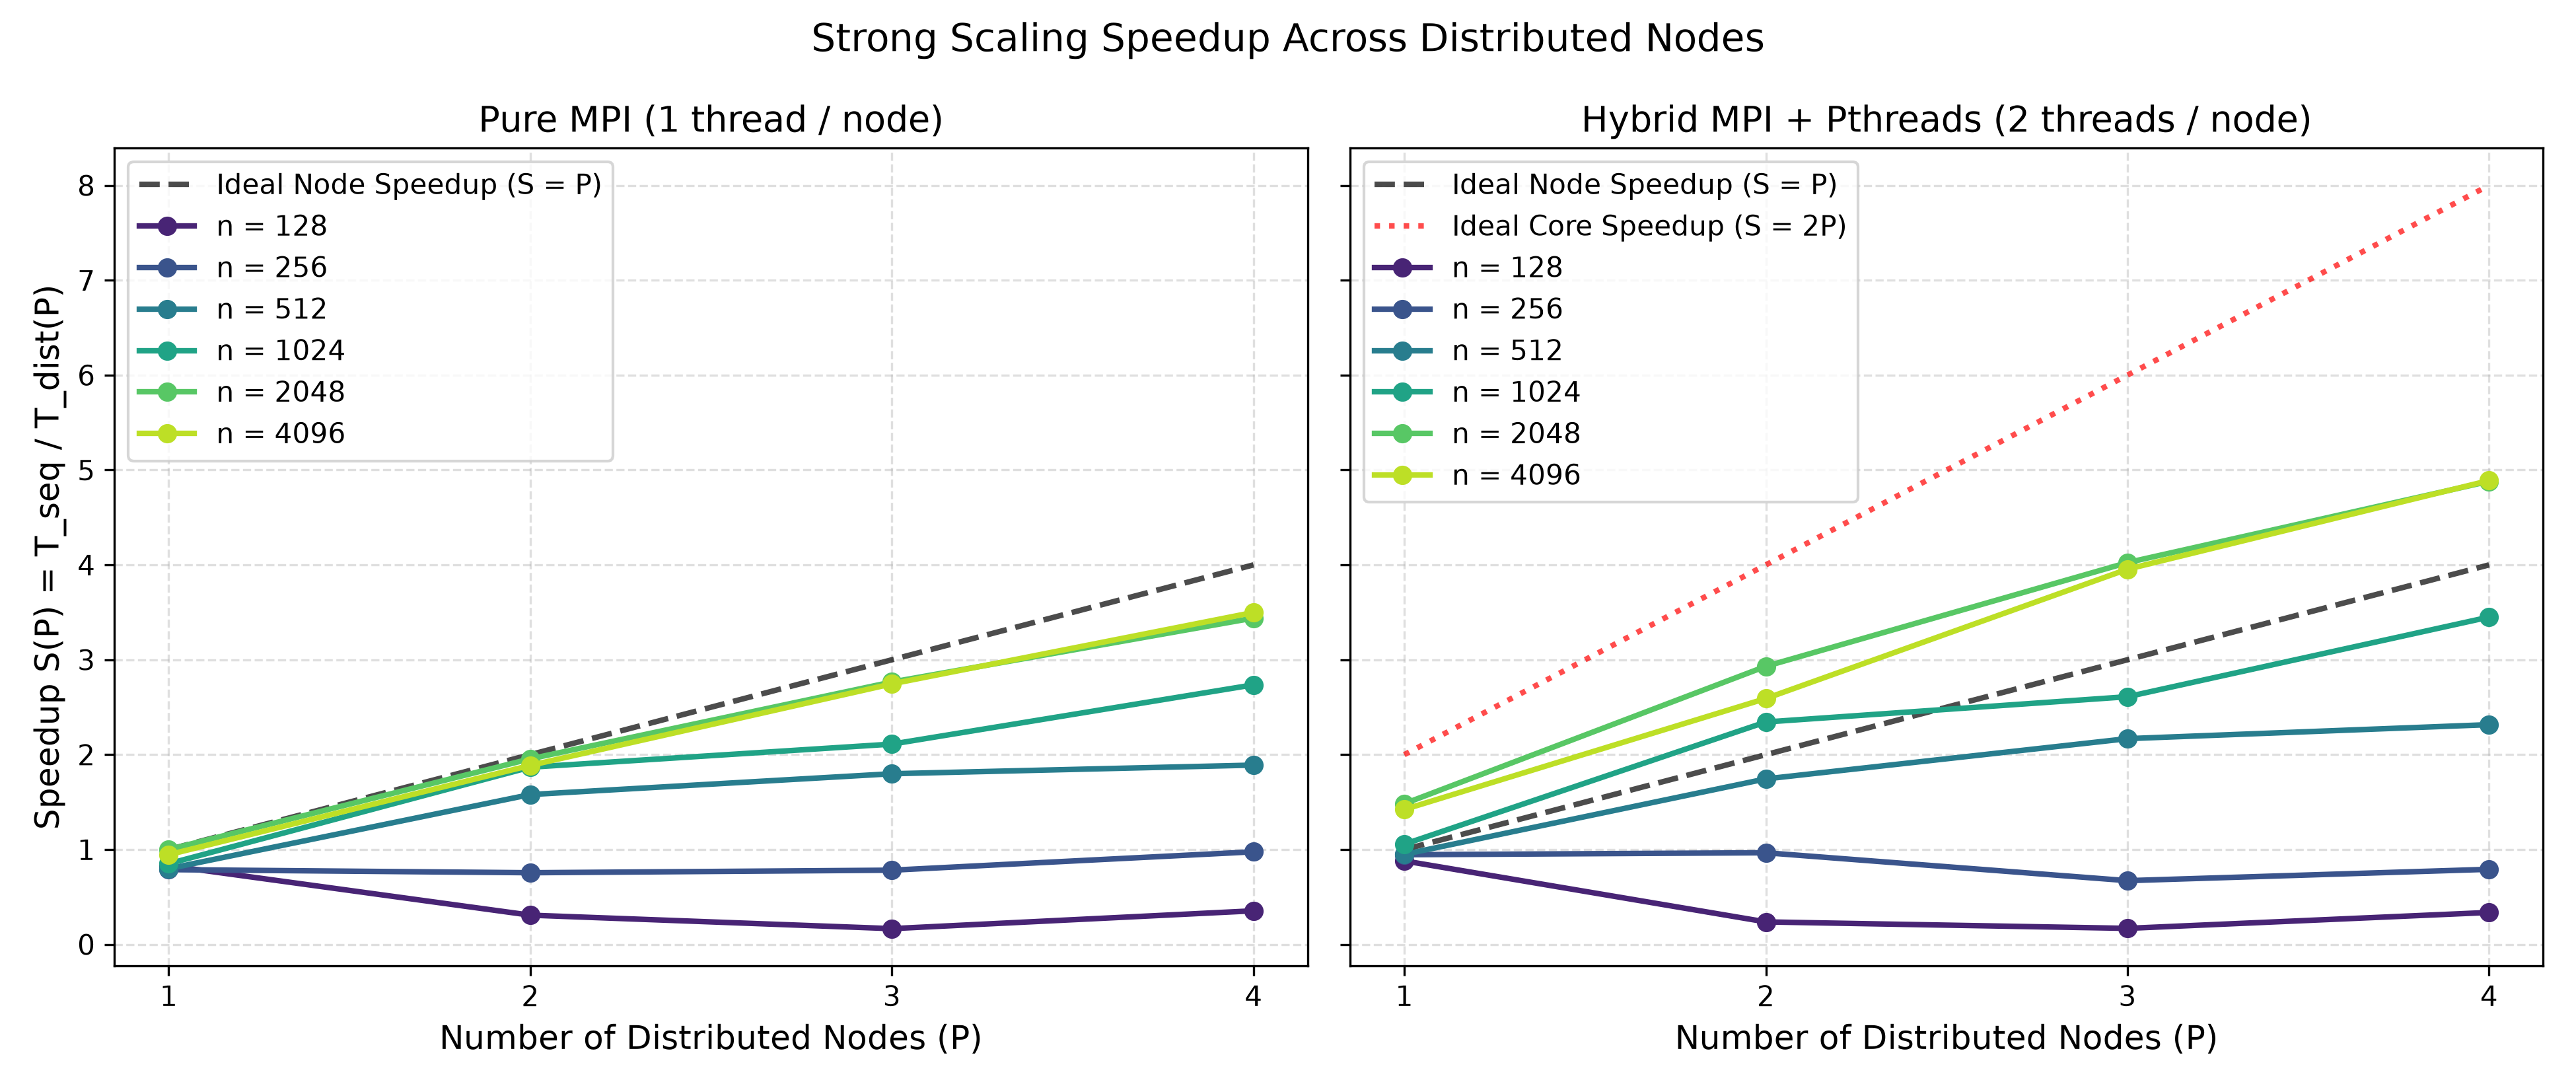
\includegraphics[width=0.92\textwidth]{results/figures/strong_scaling_speedup.png}
\caption{Strong scaling speedup $S(P)$ across $P = 1 \dots 4$ nodes for Pure MPI and Hybrid MPI+Pthreads.}
\label{fig:speedup}
\end{figure}

\begin{figure}[htbp]
\centering
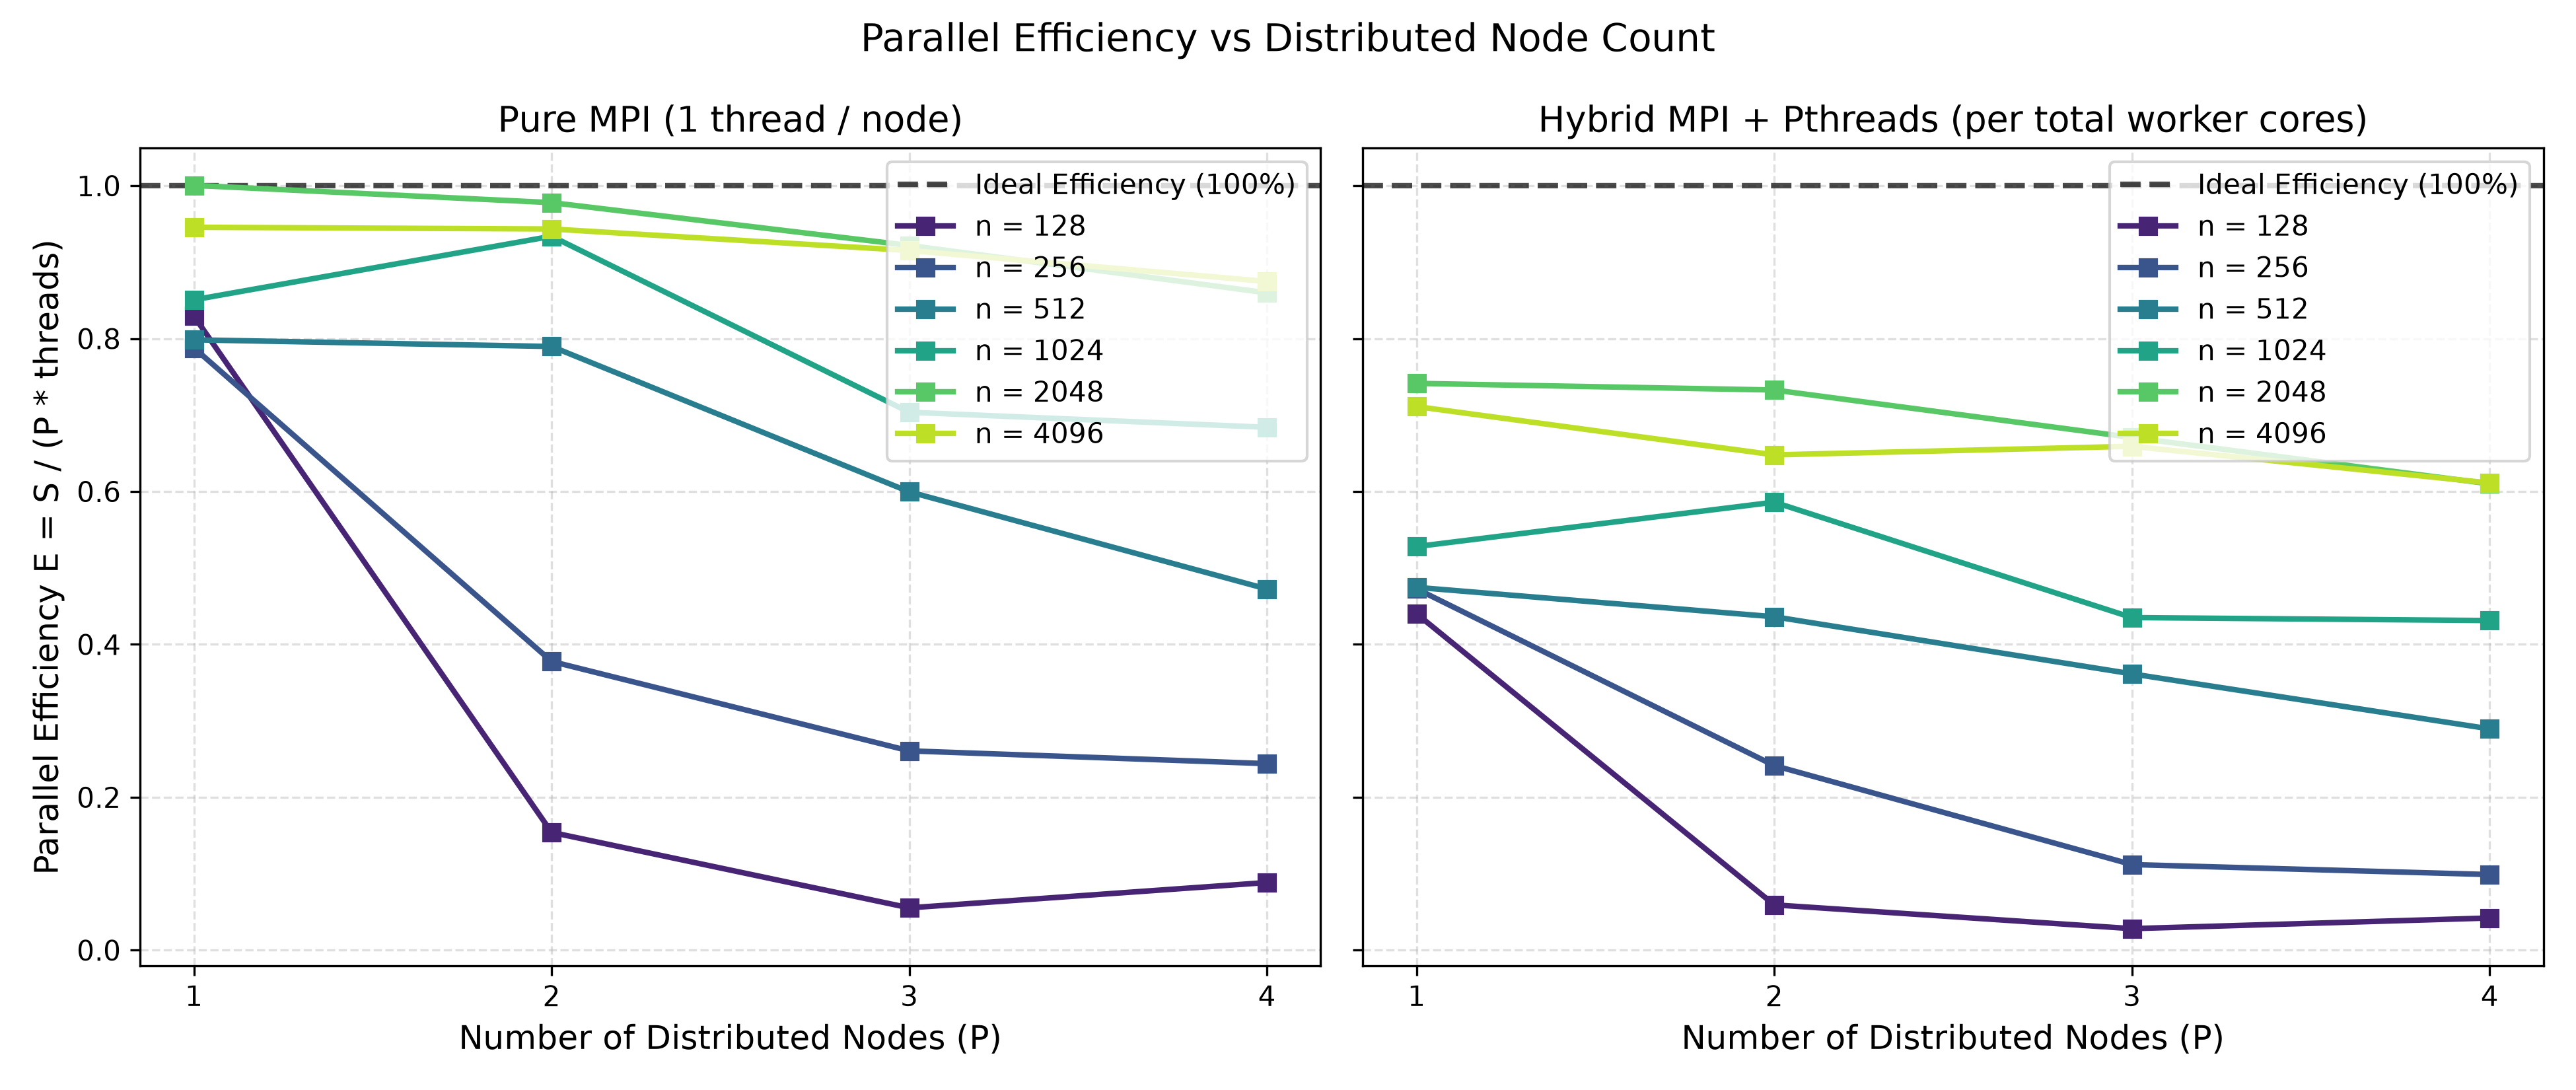
\includegraphics[width=0.92\textwidth]{results/figures/strong_scaling_efficiency.png}
\caption{Parallel efficiency $E = S / (P \times \text{threads})$ across $P = 1 \dots 4$ distributed nodes.}
\label{fig:efficiency}
\end{figure}

The results show three clear regimes:
\begin{itemize}
    \item \textbf{Small matrices ($n \le 256$):} Distributed execution is slower than running sequentially on 1 core. At $n = 128$, 4 nodes only achieve a speedup of $0.35\times$ ($2.24\text{ ms}$ vs.\ $0.79\text{ ms}$ sequential). At $n = 256$, 4 nodes reach $0.98\times$ ($6.12\text{ ms}$ vs.\ $5.97\text{ ms}$), which is the break-even point.
    \item \textbf{Near-linear Pure MPI scaling on large matrices ($n \ge 1024$):} At $n = 4096$, sequential execution takes \textbf{58.77 seconds} (IQR: $0.59\text{ s}$). With Pure MPI (1 thread per node = 1 physical core per VM), runtime drops to \textbf{31.15s} at $P = 2$ ($1.89\times$ speedup, $94.4\%$ efficiency), \textbf{21.40s} at $P = 3$ ($2.75\times$ speedup, $91.5\%$ efficiency), and \textbf{16.80s} at $P = 4$ (\textbf{3.50$\times$ speedup}, $87.5\%$ efficiency). If we look only at the computation phase ($15.56\text{ s}$ at $P = 4$), the compute speedup is $3.78\times$ out of $4.0\times$.
    \item \textbf{Hybrid MPI + Pthreads improvement:} Adding 2 POSIX threads per node uses both Hyper-Threads of each VM's Xeon core. On 1 node, \texttt{par\_ikj} (2 threads) reduces runtime at $n = 4096$ from $58.77\text{ s}$ to $40.26\text{ s}$ ($1.46\times$ speedup). Across 4 nodes (8 total vCPUs), \texttt{mpi\_hybrid} reduces runtime to \textbf{12.02 seconds} (IQR: $0.78\text{ s}$), achieving a \textbf{4.89$\times$ total speedup} over the sequential baseline.
\end{itemize}

\subsection{Runtime Comparison and Communication Breakdown (RQ2)}
Figure~\ref{fig:exec_time} compares the log-log execution time across all matrix sizes for \texttt{seq\_ikj}, single-node \texttt{par\_ikj}, 4-node \texttt{mpi\_ikj}, and 4-node \texttt{mpi\_hybrid}. Figure~\ref{fig:comm_breakdown} breaks down the 4-node execution time into data distribution, local computation, and result collection.

\begin{figure}[htbp]
\centering
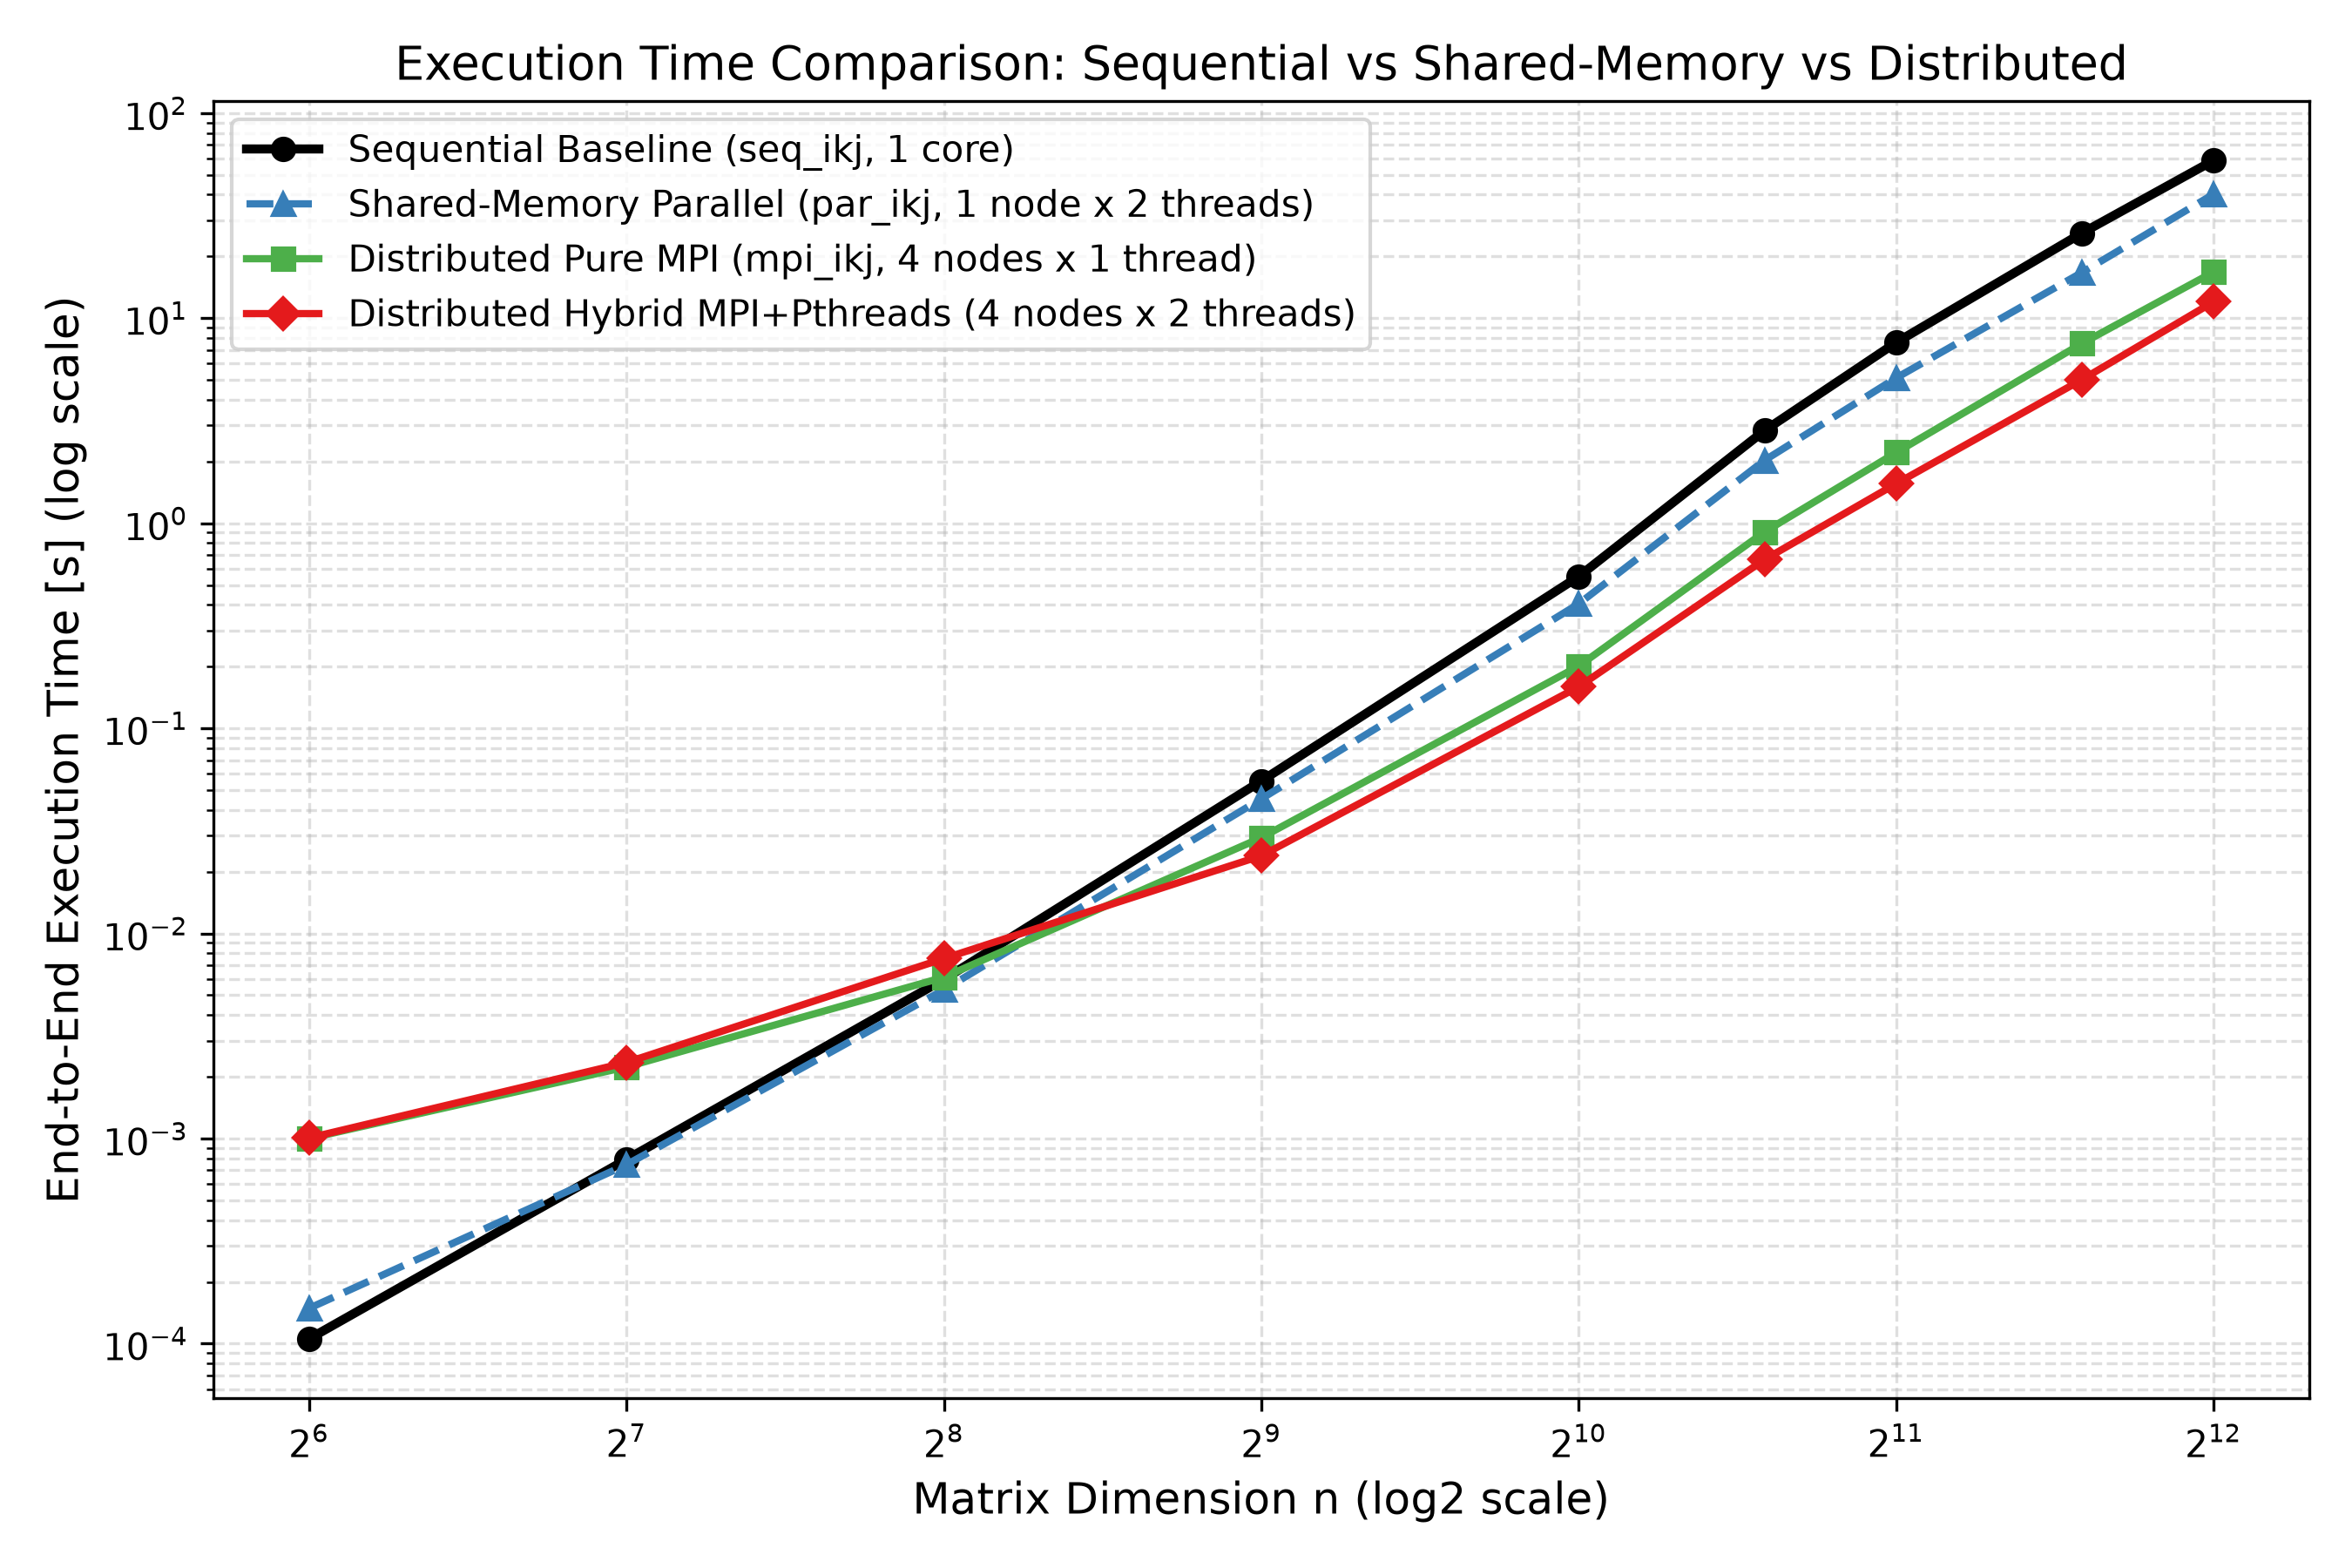
\includegraphics[width=0.68\textwidth]{results/figures/execution_time_vs_n.png}
\caption{End-to-end execution time comparison across methods ($\log_2$--$\log_2$ scale).}
\label{fig:exec_time}
\end{figure}

\begin{figure}[htbp]
\centering
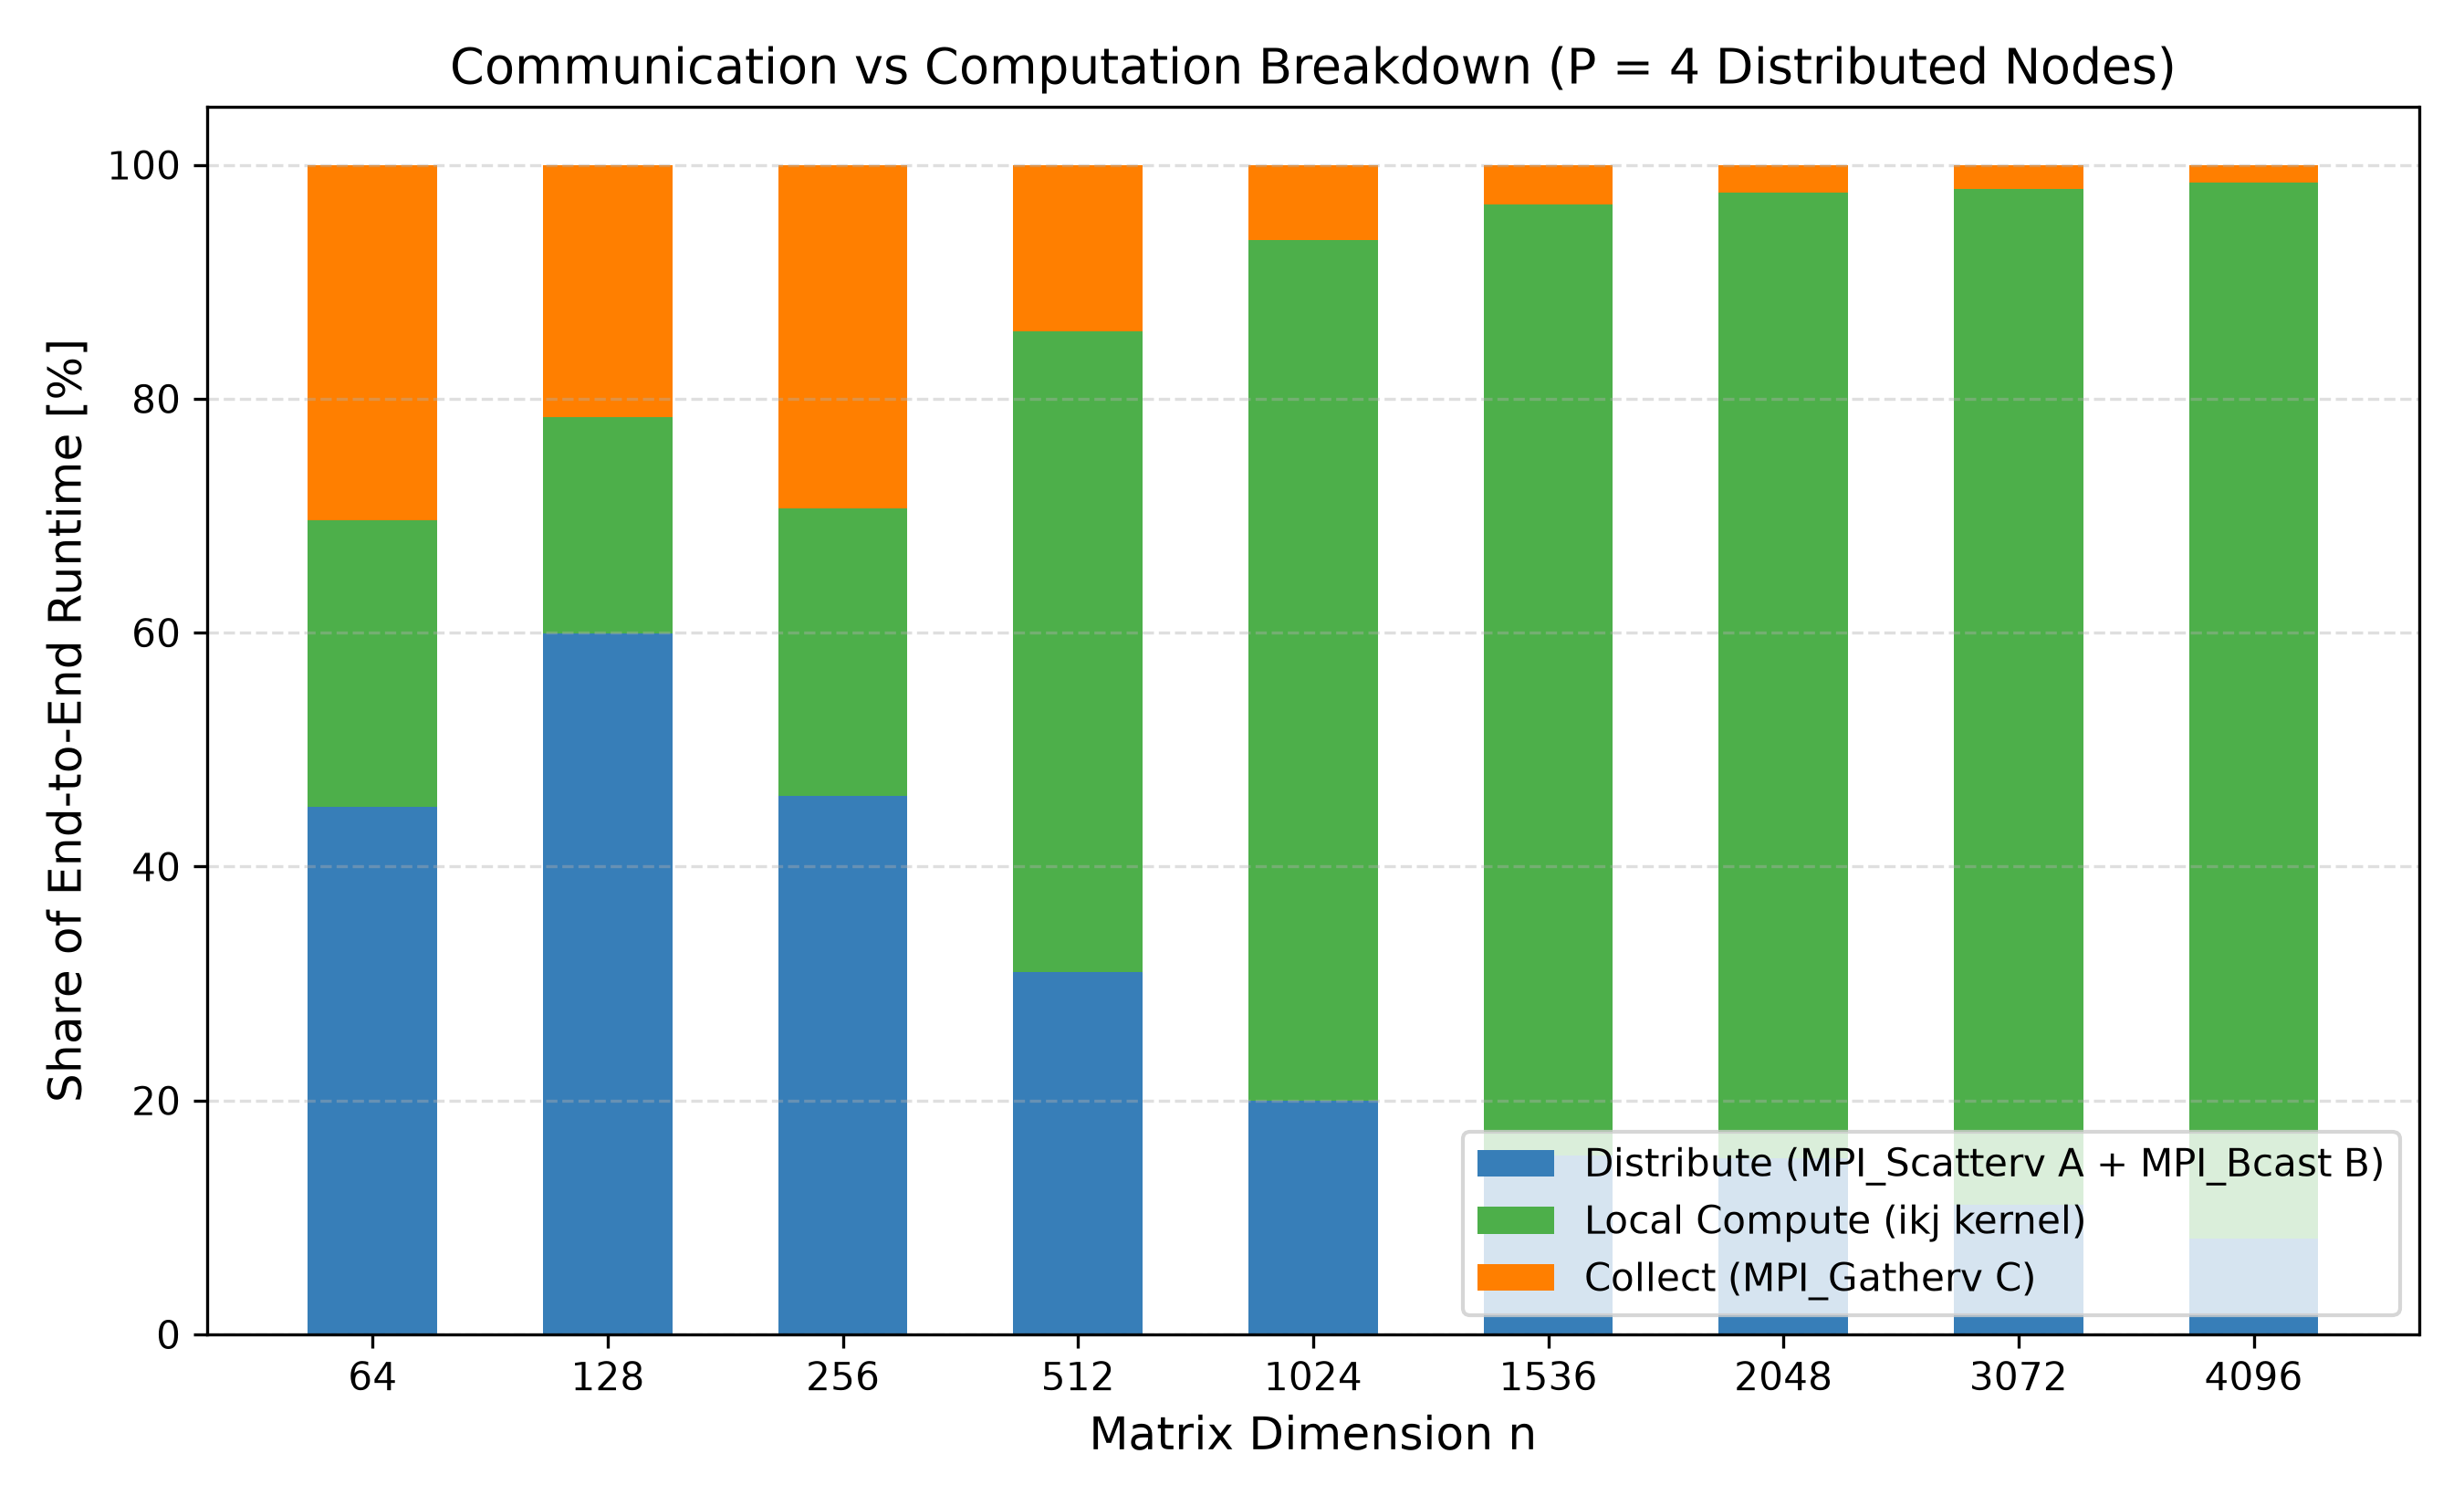
\includegraphics[width=0.68\textwidth]{results/figures/communication_breakdown.png}
\caption{Percentage of runtime spent in Distribution, Local Compute, and Collection at $P = 4$ nodes.}
\label{fig:comm_breakdown}
\end{figure}

Figure~\ref{fig:comm_breakdown} clearly explains why the curves in Figure~\ref{fig:exec_time} cross between $n = 256$ and $n = 512$:
\begin{itemize}
    \item At $n = 64$ and $n = 128$, network communication (\texttt{Scatterv} + \texttt{Bcast} + \texttt{Gatherv}) consumes \textbf{75\% to 81\%} of the total execution time, while actual multiplication takes less than $25\%$.
    \item Because network data volume grows quadratically as $\mathcal{O}(n^2)$ while matrix multiplication arithmetic grows cubically as $\mathcal{O}(n^3)$, the communication percentage drops rapidly as $n$ increases: at $n = 512$ communication is $45.4\%$, at $n = 1024$ it is $26.5\%$, and at $n = 2048$ it is $17.4\%$.
    \item At $n = 4096$ ($P = 4$, transferring $604.0\text{ MB}$ in total across the cluster), local computation accounts for \textbf{90.3\%} of the runtime ($10.85\text{ s}$), distributing $A$ and $B$ takes \textbf{8.2\%} ($0.98\text{ s}$), and gathering $C$ takes only \textbf{1.5\%} ($0.18\text{ s}$). Distribution takes longer than collection because \texttt{MPI\_Bcast} must send the entire $128\text{ MiB}$ matrix $B$ to every worker, whereas \texttt{MPI\_Gatherv} only collects $\frac{3}{4}$ of matrix $C$ ($96\text{ MiB}$ total).
\end{itemize}

\subsection{Memory Scaling Per Node and Across the Cluster (RQ3)}
Figure~\ref{fig:memory} compares the Peak RSS of Rank 0, the maximum Peak RSS among worker nodes (Ranks 1--3), the total cluster RSS across all 4 nodes, and the theoretical single-node footprint ($3 \times 8n^2$).

\begin{figure}[htbp]
\centering
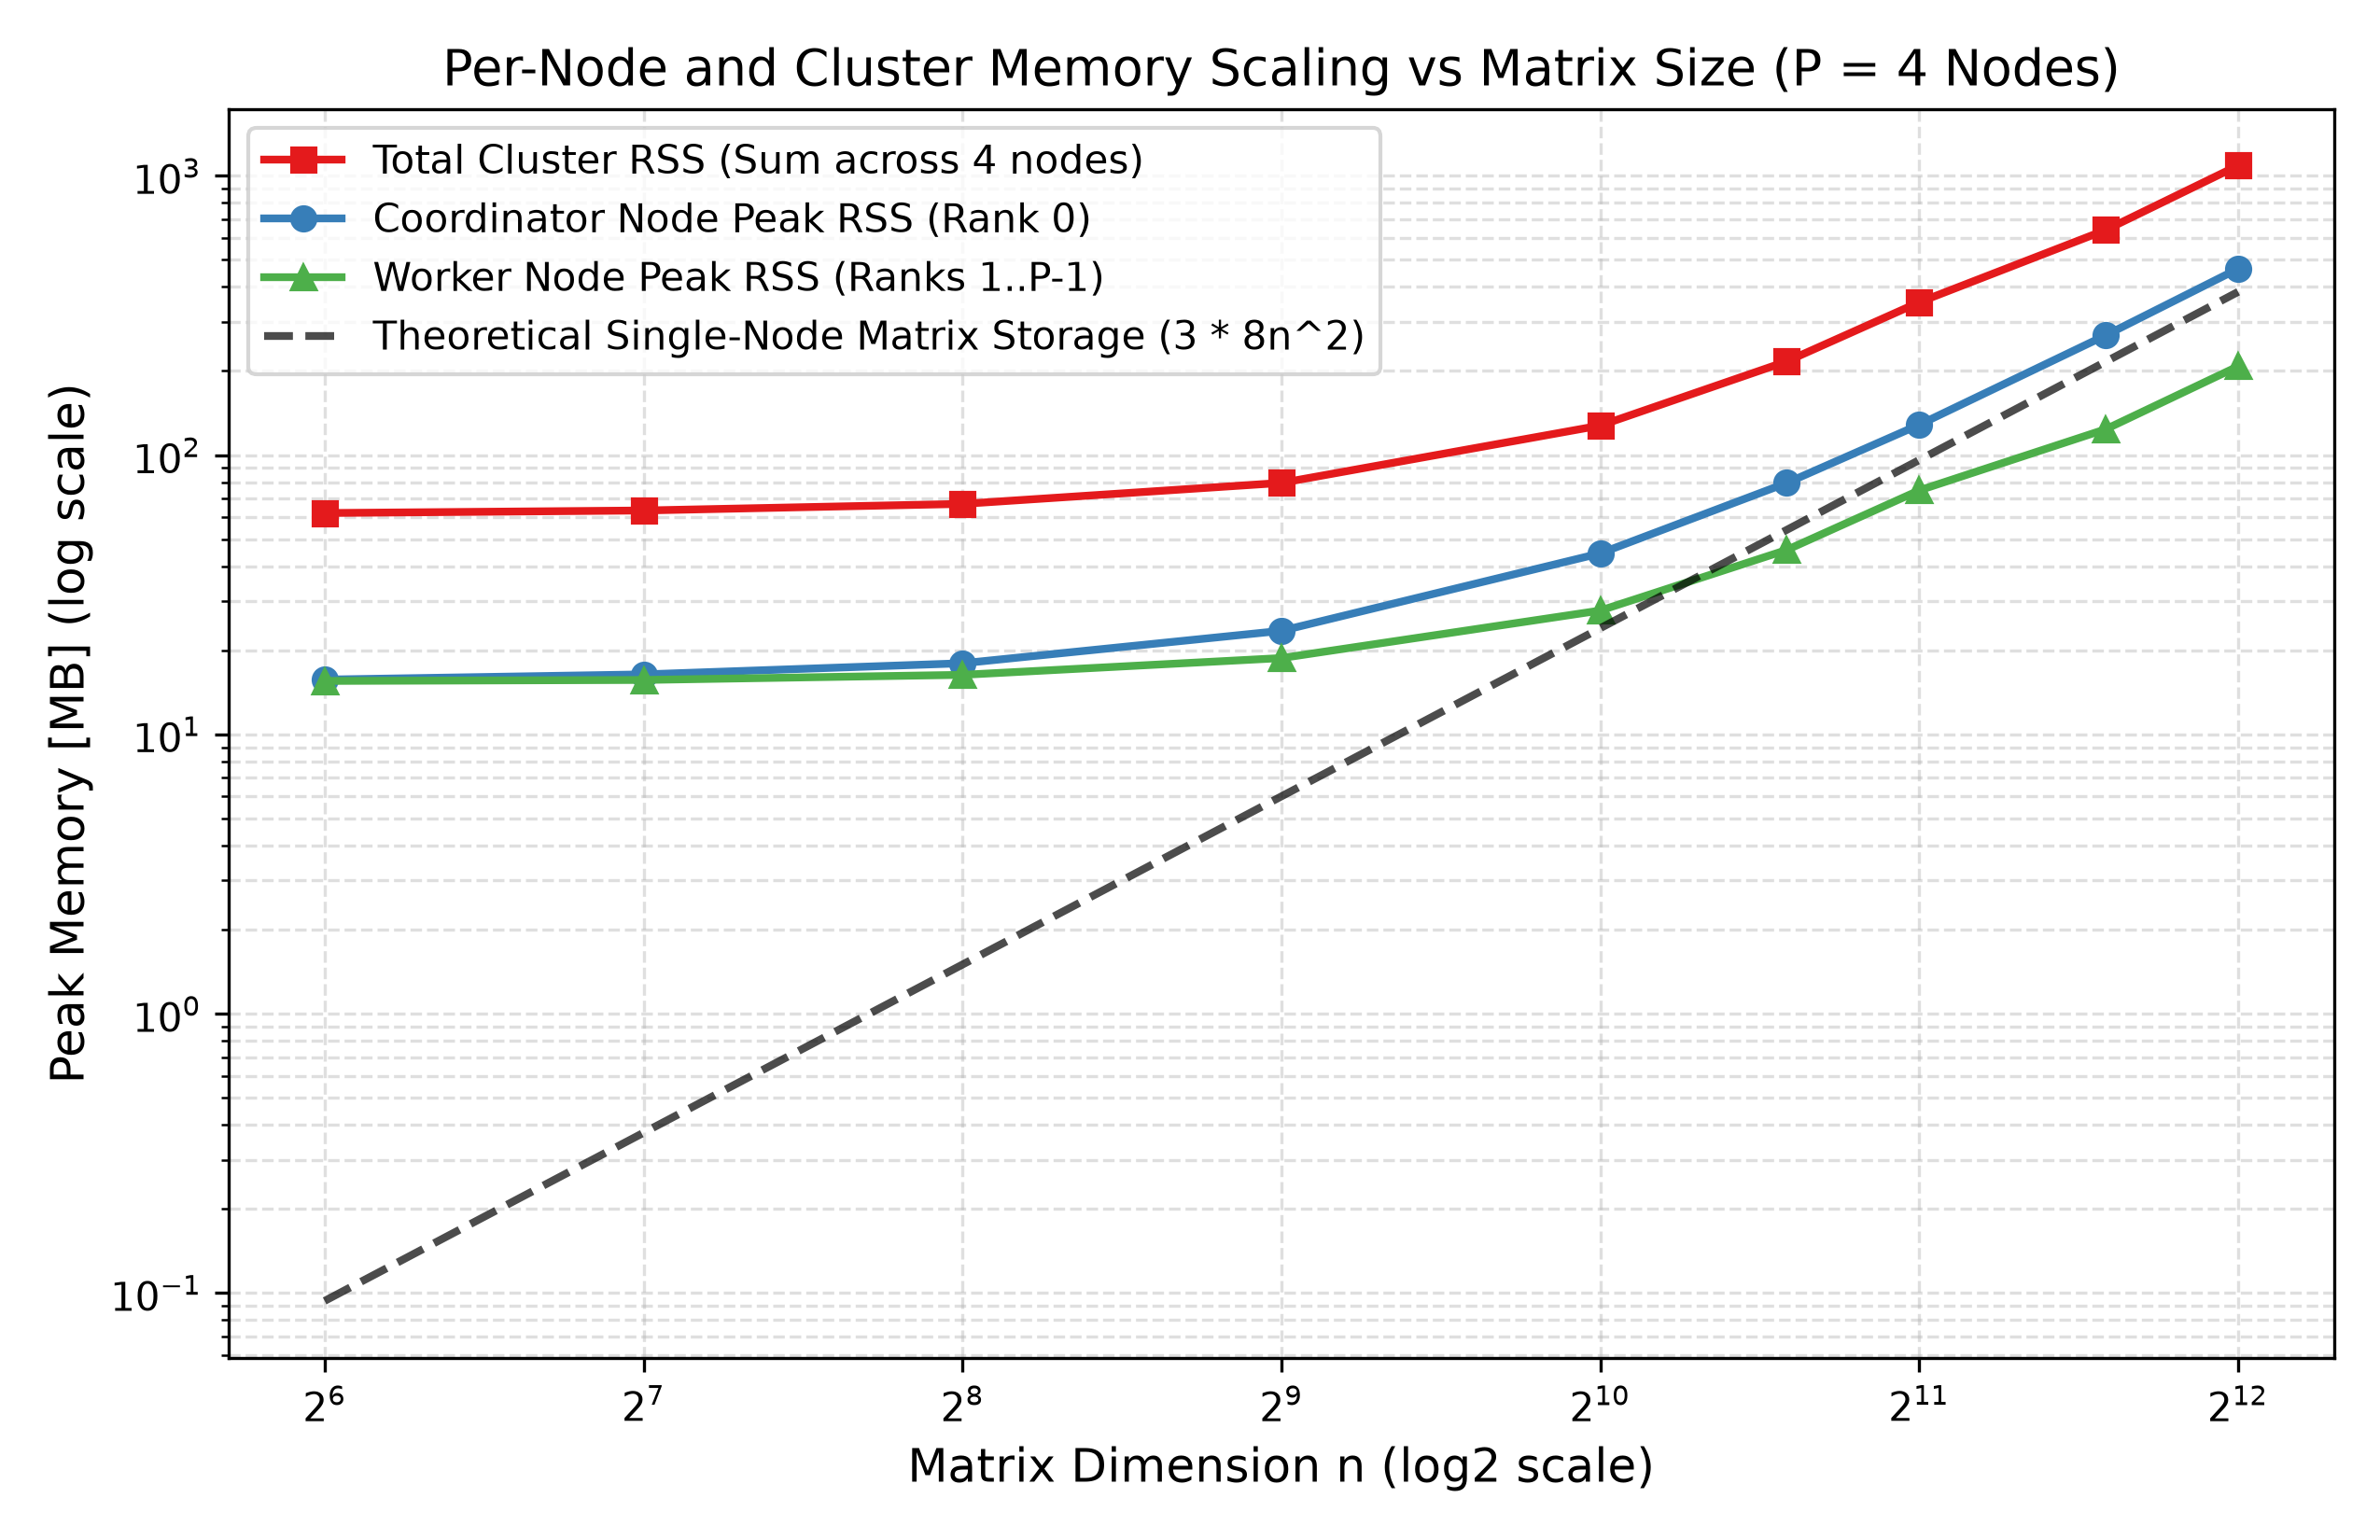
\includegraphics[width=0.68\textwidth]{results/figures/memory_scaling.png}
\caption{Per-node and total cluster Peak RSS versus matrix size $n$ at $P = 4$ nodes.}
\label{fig:memory}
\end{figure}

\begin{itemize}
    \item \textbf{Base MPI Overhead ($n \le 256$):} While sequential \texttt{seq\_ikj} uses only $0.7\text{ MB}$ at $n = 64$, each OpenMPI process has a base memory footprint of $\sim 15.5\text{ MB}$ for network buffers and shared libraries.
    \item \textbf{Worker Memory Reduction ($n = 4096$):} On a single node, storing three $4096 \times 4096$ matrices requires $384.0\text{ MiB}$ (measured \texttt{seq\_ikj} RSS: $384.8\text{ MiB}$). With $P = 4$ nodes, each worker node only allocates $\frac{1}{4}$ of $A$ ($32\text{ MiB}$), the full matrix $B$ ($128\text{ MiB}$), and $\frac{1}{4}$ of $C$ ($32\text{ MiB}$), resulting in a measured worker Peak RSS of \textbf{207.9 MiB}---almost half the memory of a single-node run.
    \item \textbf{Coordinator and Total Cluster Memory:} Rank 0 uses \textbf{464.6 MiB} because it holds the full matrices $A, B, C$ ($384\text{ MiB}$) plus its temporary local slices ($64\text{ MiB}$). Summing all 4 nodes gives a total cluster footprint of \textbf{1088.0 MiB}, because matrix $B$ is replicated across all 4 machines.
\end{itemize}

\subsection{Weak Scaling Analysis (RQ4)}
Figure~\ref{fig:weak} evaluates weak scaling where total arithmetic work per node ($2n^3 / P$) is kept constant by setting $n = 1024, 1290, 1477, 1625$ for $P = 1, 2, 3, 4$.

\begin{figure}[htbp]
\centering
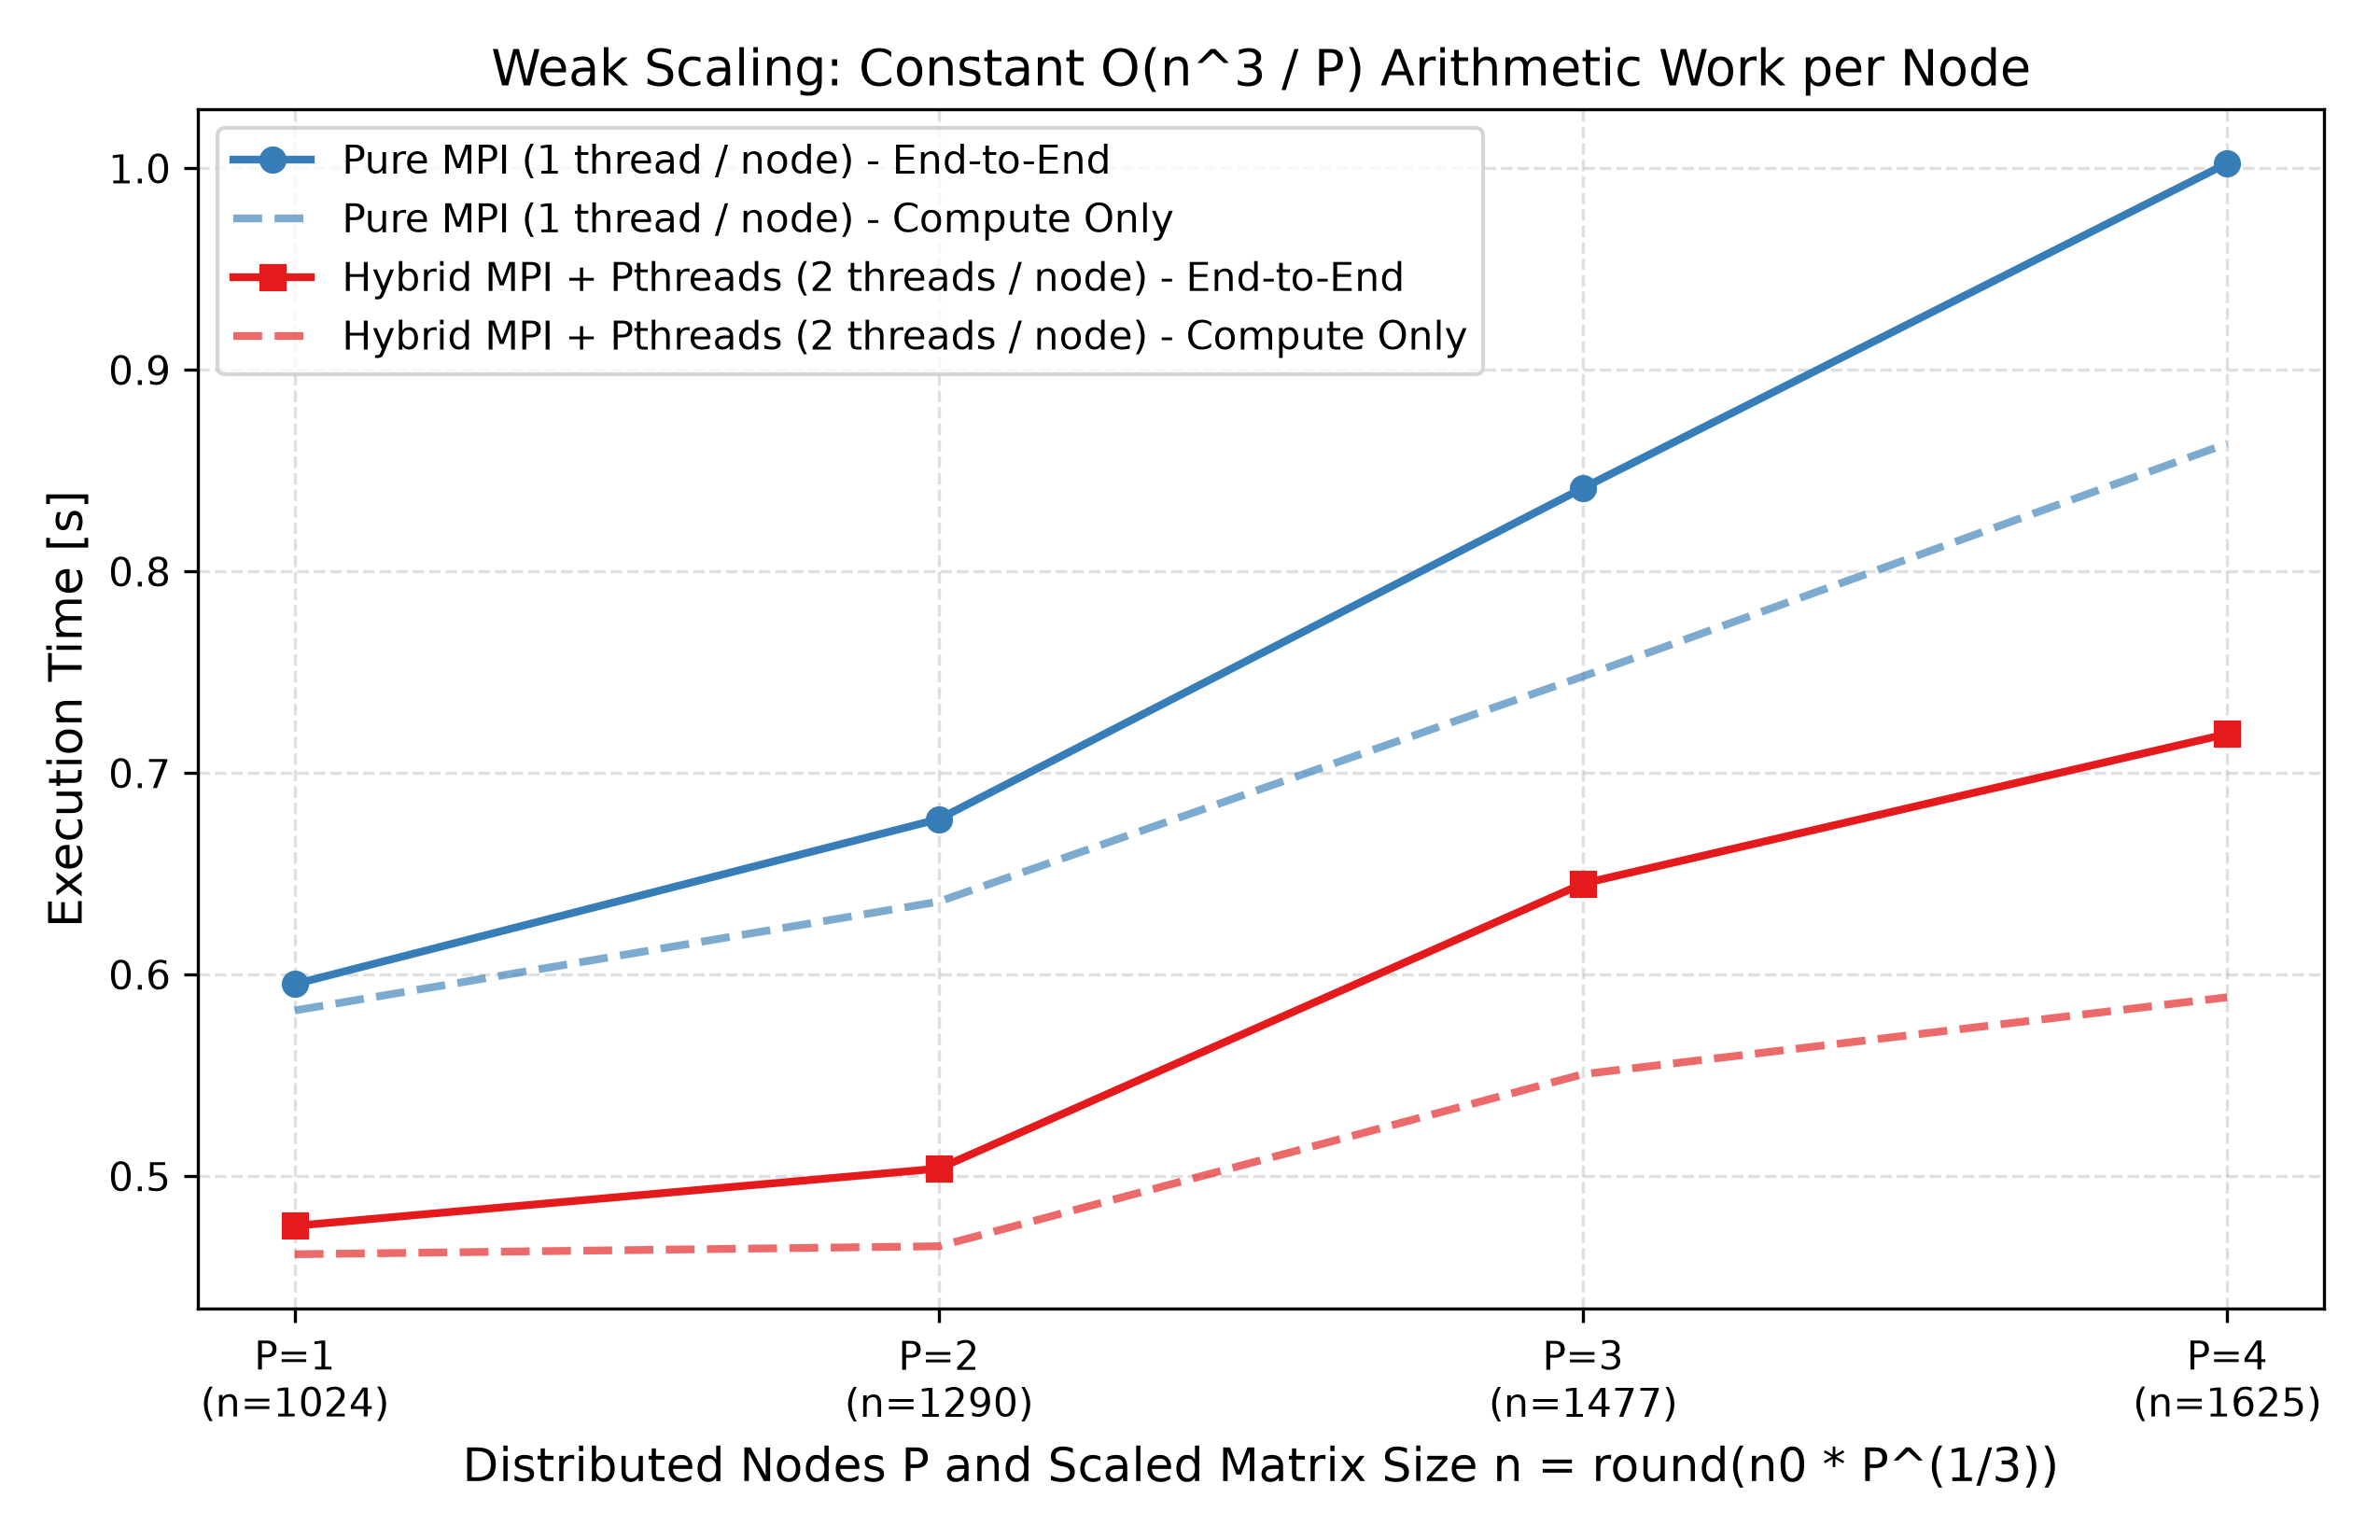
\includegraphics[width=0.68\textwidth]{results/figures/weak_scaling.png}
\caption{Weak scaling runtime (end-to-end vs.\ compute-only) under constant $\mathcal{O}(n^3 / P)$ work per node.}
\label{fig:weak}
\end{figure}

Looking at the dashed compute-only lines, local computation time stays very flat between $P = 1$ ($0.461\text{ s}$ for hybrid) and $P = 2$ ($0.465\text{ s}$), rising slightly to $0.589\text{ s}$ at $P = 4$ as the larger matrix $B$ ($n = 1625$, $20.1\text{ MiB}$) begins exceeding fast cache levels. The solid end-to-end curve rises from $0.475\text{ s}$ ($P = 1$) to $0.719\text{ s}$ ($P = 4$) primarily because total network data transferred increases from $0\text{ MB}$ at $P = 1$ to $95.0\text{ MB}$ at $P = 4$ ($0.109\text{ s}$ of distribution + $0.024\text{ s}$ of collection).

\section{Discussion and Comparison with Previous Assignments}

Comparing the distributed cluster results against my Assignment 3 shared-memory results highlights the fundamental differences between shared-memory and distributed-memory computing:

\begin{enumerate}
    \item \textbf{Parallelism Threshold ($n > 128$ vs.\ $n > 256$):} In Assignment 3 on my laptop, shared-memory threads beat sequential execution starting at $n = 128$ because waking up threads in the same memory space takes only a few microseconds. In Assignment 4 across 4 cloud VMs, distributed execution only beats sequential execution at $n \ge 512$ (breaking even at $n = 256$) because serializing and sending megabytes of data over TCP/IP sockets is much slower than passing a pointer in shared RAM.
    \item \textbf{Scaling Efficiency Across Physical Cores:} On my heterogeneous laptop in Assignment 3 (4 P-cores + 8 E-cores, 16 threads sharing one memory bus), efficiency dropped to $32.4\%$ at 16 threads ($5.19\times$ speedup) due to E-core asymmetry and shared RAM bandwidth saturation. In contrast, our 4 homogeneous cloud VMs each have their own independent RAM bus and Xeon physical core, allowing Pure MPI to reach a very high \textbf{87.5\% efficiency} ($3.50\times$ on 4 cores), and Hybrid MPI+Pthreads to reach \textbf{4.89$\times$ on 8 vCPUs} (since each VM's second vCPU is a Hyper-Thread sharing the same physical core, contributing an extra $\sim 39\%$ throughput boost).
    \item \textbf{Limitations of the Study:} First, Rank 0 holds the full input and output matrices in memory, meaning the maximum matrix size is still bounded by Rank 0's $1.9\text{ GiB}$ RAM ($n = 4096$ used $464.6\text{ MiB}$ on Rank 0). Processing matrices larger than one machine's memory would require distributed file I/O (MPI-IO) and a 2D block algorithm such as SUMMA so no single node ever holds all of $A$, $B$, or $C$. Second, each \texttt{e2-highcpu-2} VM provides 1 physical core with 2 SMT threads rather than 2 independent physical cores, which caps the intra-node Pthreads gain at $\sim 1.46\times$.
\end{enumerate}

\section{Conclusions}

Within the tested scope of a 4-node Google Cloud cluster ($4 \times \text{e2-highcpu-2}$, $n = 64 \dots 4096$), this study establishes the following conclusions:

\begin{enumerate}
    \item \textbf{Strong scaling is highly effective for large matrices (RQ1):} At $n = 4096$, Pure MPI across 4 nodes achieves a \textbf{3.50$\times$ speedup} ($87.5\%$ efficiency), and Hybrid MPI + Pthreads (4 nodes $\times$ 2 threads) achieves a \textbf{4.89$\times$ speedup}, reducing execution time from $58.77\text{ s}$ down to $12.02\text{ s}$.
    \item \textbf{Cubic compute quickly outgrows quadratic network transfer (RQ2):} Network communication dominates small matrices ($>70\%$ of runtime for $n \le 256$), making distribution slower than 1 local core. By $n = 4096$, network transfer represents only $9.7\%$ of total runtime ($0.98\text{ s}$ distribute + $0.18\text{ s}$ gather vs.\ $10.85\text{ s}$ compute).
    \item \textbf{1D row partitioning halves worker memory but increases total cluster memory (RQ3):} At $n = 4096$, worker node memory drops to $207.9\text{ MiB}$ (vs.\ $384.8\text{ MiB}$ sequential), while broadcasting $B$ to all nodes raises aggregate cluster memory across the 4 VMs to $1088.0\text{ MiB}$.
    \item \textbf{Weak scaling maintains stable compute times (RQ4):} Scaling $n \propto P^{1/3}$ keeps per-node compute time nearly flat ($0.46\text{ s}\text{--}0.59\text{ s}$), with end-to-end runtime increasing modestly due to growing $\mathcal{O}(n^2)$ broadcast volume.
\end{enumerate}

\section*{Declaration on the Use of Artificial Intelligence}

In accordance with the course's academic integrity policy, I declare that I used an AI assistant (\textbf{Google Antigravity}) during the development of this assignment.

The tool was used in the following specific areas:
\begin{enumerate}
    \item \textbf{Explanation and Conceptual Discussion:} I used the AI assistant to understand distributed-memory programming with OpenMPI, how collective MPI calls (\texttt{Scatterv}, \texttt{Bcast}, and \texttt{Gatherv}) work compared to shared-memory threads, and how to set up a multi-node cluster on Google Cloud Platform.
    \item \textbf{Planning and Implementation Structure:} I consulted the AI to design the 1D row-partitioning module (\texttt{src/mpi\_matmul.c}) and the hybrid integration with my Assignment 3 POSIX thread pool, as well as the phase-isolated benchmarking harness and plotting script.
    \item \textbf{Debugging and Verification:} The AI assisted in building the distributed unit test suite (\texttt{tests/test\_mpi.c}) and troubleshooting OpenMPI SSH host-key and slot configuration on the Google Cloud virtual machines.
    \item \textbf{Language Revision and Formatting:} The AI helped revise the English phrasing and \LaTeX{} formatting of this report.
\end{enumerate}

\textbf{Student Responsibility and Verification:}
All experimental benchmarks reported in this study were executed on a real 4-node Google Cloud cluster configured by me, and all figures and conclusions come directly from those empirical CSV measurements. I personally reviewed, understood, and validated the code and results, and I take full responsibility for defending this work.

\end{document}
